%% -*- coding: utf-8 -*-
\documentclass[12pt,a4paper]{scrartcl} 
\usepackage[utf8]{inputenc}
\usepackage[english,russian]{babel}
\usepackage{indentfirst}
\usepackage{misccorr}
\usepackage{graphicx}
\usepackage{amsmath}
\usepackage{listings}
\usepackage{color}
\usepackage{float}

\definecolor{gray}{rgb}{0.5,0.5,0.5}
\definecolor{mauve}{rgb}{0.58,0,0.82}
\definecolor{lightgray}{rgb}{.9,.9,.9}
\definecolor{green}{rgb}{.2,.7,.1}
\definecolor{orange}{rgb}{.7,.3,.1}
\definecolor{purple}{rgb}{0.65, 0.12, 0.82}

\lstdefinelanguage{TypeScript}{
  keywords={typeof, new, true, false, catch, function, return, null, catch, switch, var, if, in, while, do, else, case, break, const, number, string, boolean, void, array},
  keywordstyle=\color{blue}\bfseries,
  ndkeywords={class, export, boolean, throw, implements, import, this, constructor, get, set, private},
  ndkeywordstyle=\color{green}\bfseries,
  identifierstyle=\color{black},
  numberstyle=\tiny\color{gray},
  sensitive=false,
  comment=[l]{//},
  morecomment=[s]{/*}{*/},
  commentstyle=\color{lightgray}\ttfamily,
  stringstyle=\color{orange}\ttfamily,
  morestring=[b]',
  morestring=[b]"
}

\lstdefinestyle{ts-style}{
  frame=tb,
  language=TypeScript,
  aboveskip=3mm,
  belowskip=3mm,
  showstringspaces=false,
  columns=flexible,
  basicstyle={\small\ttfamily},
  numbers=none,
  breaklines=true,
  breakatwhitespace=true,
  tabsize=3
}

\begin{document}
\begin{titlepage}
		\begin{center}
			\large
			МИНИСТЕРСТВО НАУКИ И ВЫСШЕГО ОБРАЗОВАНИЯ РОССИЙСКОЙ ФЕДЕРАЦИИ
			
			Федеральное государственное бюджетное образовательное учреждение высшего образования
			
			\textbf{АДЫГЕЙСКИЙ ГОСУДАРСТВЕННЫЙ УНИВЕРСИТЕТ}
			\vspace{0.25cm}
			
			Инженерно-физический факультет
			
			Кафедра автоматизированных систем обработки информации и управления
			\vfill

			\vfill
			
			\textsc{Отчет по практике}\\[5mm]
			
			{\LARGE Программная реализация численного метода \textit{Решение системы линейных алгебраических уравнений методом Гаусса}}
			\bigskip
			
			1 курс, группа 1ИВТ АСОИУ
		\end{center}
		\vfill
		
		\newlength{\ML}
		\settowidth{\ML}{«\underline{\hspace{0.7cm}}» \underline{\hspace{2cm}}}
		\hfill\begin{minipage}{0.5\textwidth}
			Выполнил:\\
			\underline{\hspace{\ML}} В.\,А.~Косицкий\\
			«\underline{\hspace{0.7cm}}» \underline{\hspace{2cm}} 2024 г.
		\end{minipage}%
		\bigskip
		
		\hfill\begin{minipage}{0.5\textwidth}
			Руководитель:\\
			\underline{\hspace{\ML}} С.\,В.~Теплоухов\\
			«\underline{\hspace{0.7cm}}» \underline{\hspace{2cm}} 2024 г.
		\end{minipage}%
		\vfill
		
		\begin{center}
			Майкоп, 2024 г.
		\end{center}
	\end{titlepage}



\section{Введение}
\label{sec:intro}
\subsection{Текстовая формулировка задачи (Вариант 3)}
	Написать программу для решения системы линейных алгебраических уравнений методом Гаусса.
	
 \subsection{Теория метода}

Метод Гаусса — классический метод решения системы линейных алгебраических уравнений (Рис. ~\ref{eq:genericlinearsys}). Это метод последовательного исключения переменных, когда с помощью элементарных преобразований система уравнений приводится к равносильной системе треугольного вида, из которой последовательно, начиная с последних (по номеру), находятся все переменные системы.
	
\textbf{Алгоритм решения СЛАУ методом Гаусса подразделяется на два этапа.}	

На первом этапе осуществляется так называемый прямой ход, когда путём элементарных преобразований над строками систему приводят к ступенчатой или треугольной форме, либо устанавливают, что система несовместна. А именно, среди элементов первого столбца матрицы выбирают ненулевой, перемещают его на крайнее верхнее положение перестановкой строк и вычитают получившуюся после перестановки первую строку из остальных строк, домножив её на величину, равную отношению первого элемента каждой из этих строк к первому элементу первой строки, обнуляя тем самым столбец под ним. После того, как указанные преобразования были совершены, первую строку и первый столбец мысленно вычёркивают и продолжают пока не останется матрица нулевого размера. Если на какой-то из итераций среди элементов первого столбца не нашёлся ненулевой, то переходят к следующему столбцу и проделывают аналогичную операцию.
На втором этапе осуществляется так называемый обратный ход, суть которого заключается в том, чтобы выразить все получившиеся базисные переменные через небазисные и построить фундаментальную систему решений, либо, если все переменные являются базисными, то выразить в численном виде единственное решение системы линейных уравнений. Эта процедура начинается с последнего уравнения, из которого выражают соответствующую базисную переменную (а она там всего одна) и подставляют в предыдущие уравнения, и так далее, поднимаясь по «ступенькам» наверх. Каждой строчке соответствует ровно одна базисная переменная, поэтому на каждом шаге, кроме последнего (самого верхнего), ситуация в точности повторяет случай последней строки.
		
\begin{figure}[h]
	\centering
	\[
	\left\{
	\begin{array}{lc}
		a_{11}\cdot x_{1} + a_{12}\cdot x_{1} + \cdots + a_{1n}\cdot x_{n} & (1)\\
		a_{21}\cdot x_{1} + a_{22}\cdot x_{1} + \cdots + a_{2n}\cdot x_{n} & (2)\\
		\cdots \\
		a_{m1}\cdot x_{1} + a_{m2}\cdot x_{1} + \cdots + a_{mn}\cdot x_{n} & (m)\\
	\end{array} 
	\right.
	\]	
	\caption{Общий вид системы линейных алгебраических уравнений}\label{eq:genericlinearsys}
\end{figure}

В простейшем случае алгоритм сформулирован так:

\begin{figure}[h]
	\centering
	\[
	\begin{array}{@{}clc@{}}
		(2) \rightarrow (2) - (1) \cdot (\frac{a_{21}}{a_{11}}) &:& 
		a^{'}_{22} \cdot x_{2} + a^{'}_{23} \cdot x_{3} + \cdots + a^{'}_{2n} \cdot x_{n} = b^{'}_2\\
		
		(3) \rightarrow (3) - (1) \cdot (\frac{a_{31}}{a_{11}}) &:& 
		a^{'}_{32} \cdot x_{2} + a^{'}_{33} \cdot x_{3} + \cdots + a^{'}_{3n} \cdot x_{n} = b^{'}_3\\
		
		\cdots\\
	
		(m) \rightarrow (m) - (1) \cdot (\frac{a_{m1}}{a_{11}}) &:& 
		a^{'}_{m2} \cdot x_{2} + a^{'}_{m3} \cdot x_{3} + \cdots + a^{'}_{mn} \cdot x_{n} = b^{'}_n\\
		
		(3) \rightarrow (3) - (2) \cdot (\frac{a^{'}_{32}}{a^{'}_{22}}) &:& 
		a^{''}_{33} \cdot x_{3} + \cdots + a^{''}_{3n} \cdot x_{n} = b^{''}_3\\
		
		\cdots\\
		
		(m) \rightarrow (m) - (m - 1) \cdot (\frac{a^{(m - 2)}_{m,n - 1}}{a^{m - 2}_{m - 1, n - 	1}}) &:& 
		a^{(m - 1)}_{mm} \cdot x_{m} + \cdots + a^{(m - 1)}_{mn} \cdot x_{n} = b^{(m - 1)}_m\\
	\end{array}
	\]
	\caption{Алгоритм в общем виде}\label{eq:genericlinearsysalg}
\end{figure}

Из последнего ненулевого уравнения выражаем базисную переменную через небазисные и подставляем в предыдущие уравнения. Повторяя эту процедуру для всех базисных переменных, получаем фундаментальное решение (Рис.~\ref{eq:genericlinearsysalg}).


\section{Ход работы}
\label{sec:exp}

\subsection{Выбор средств для разработки}
\label{sec:exp:selection}
Для разработки программы для решения системы линейных алгебраических уравнений методом Гаусса мной был выбран язык программирования TypeScript и фреймворк для разработки Web-приложений Angular 17. Данный стек был выбран с целью обеспечения совместимости со всеми основными операционными системами как на ПК (macOS, Windows и ОС на ядре Linux), так и с мобильными платформами (iOS и Android). Использование TypeScript позволяет организовать типобезопасность приложения, а Angular позволяет использовать привязки данных и работу по паттерну MVVM.

\subsection{Код приложения}
\label{sec:exp:code}
Для упрощения разработки было создано несколько вспомогательных классов. Листинг кода для этих классов приведён ниже:

\lstinputlisting[caption=Код класса Matrix для инкапсуляции работы с матрицами, label={lst:listing-matrix-class}, language=TypeScript, style=ts-style]{./src/app/_types/matrix.ts}

\newpage

\lstinputlisting[caption=Код класса GaussianCalculator для инкапсуляции вычисления корней СЛАУ методом Гаусса, label={lst:listing-gel-calc-class}, language=TypeScript, style=ts-style]{./src/app/_core/gaussian-calc.ts}


\section{Скриншоты программы}
\label{sec:program-shots}
Пример внешнего вида программы представлен на рис.~\ref{fig:screenshot0} и рис.~\ref{fig:screenshot1}.

\begin{figure}[H]
	\centering
	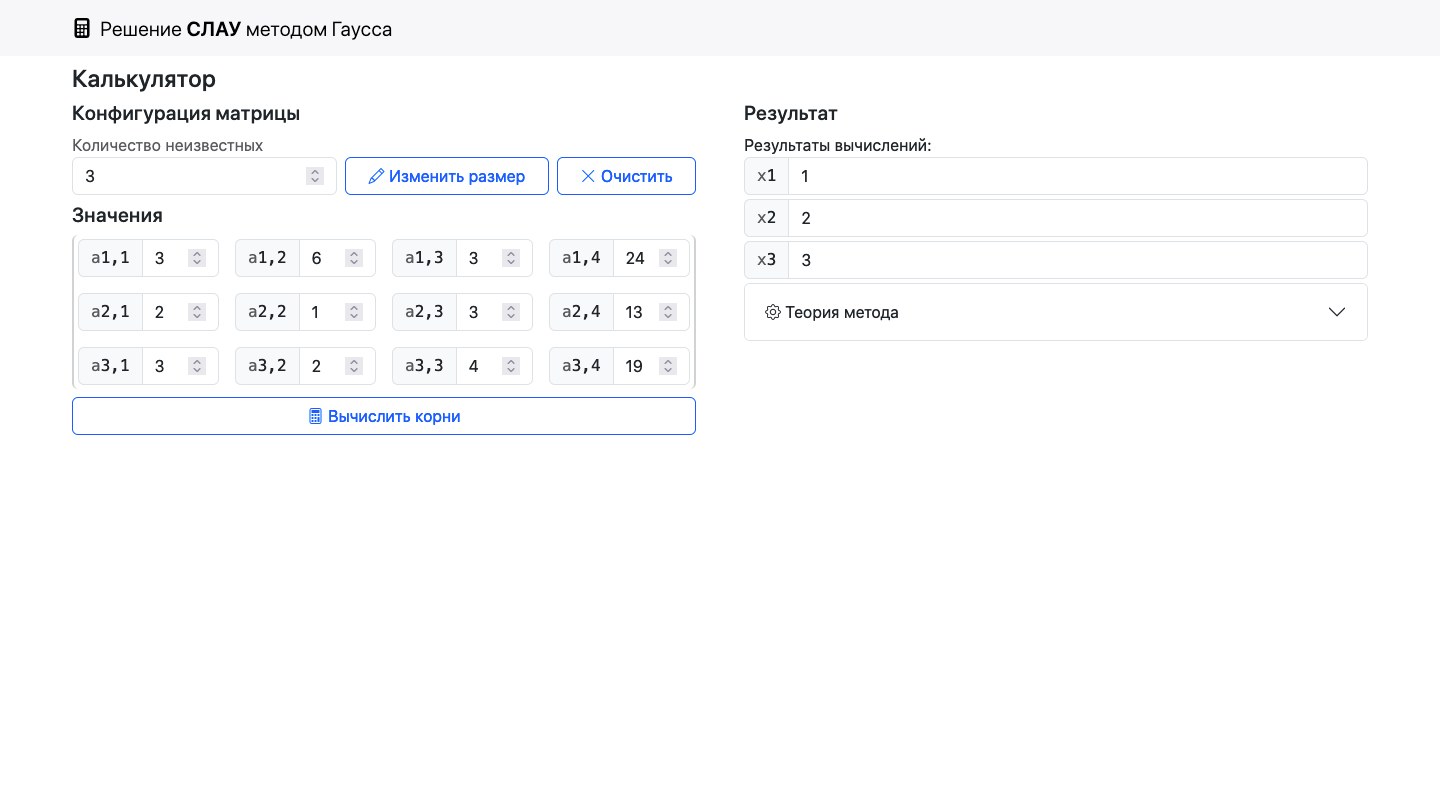
\includegraphics[width=0.85\textwidth]{./pictures/screenshot0.png}
	\caption{Внешний вид приложения на ПК}
	\label{fig:screenshot0}
\end{figure}

\begin{figure}[H]
	\centering
	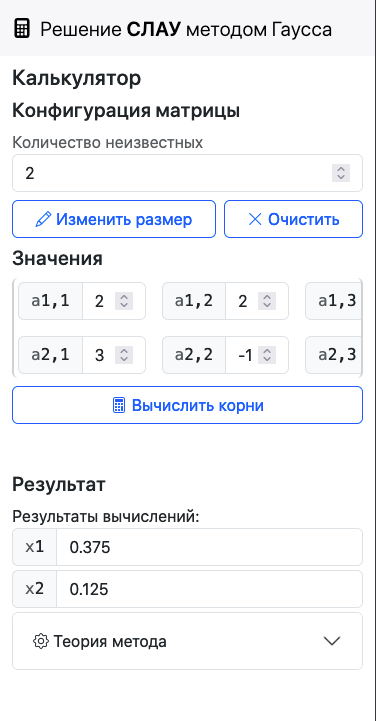
\includegraphics[width=0.4\textwidth]{./pictures/screenshot1.png}
	\caption{Внешний вид приложения на мобильных устройствах}
	\label{fig:screenshot1}
\end{figure}

\section{Источники}
\begin{thebibliography}{9}
\bibitem{Knuth-2003}Кнут Д.Э. Всё про \TeX. \newblock --- Москва: Изд. Вильямс, 2003 г. 550~с.
\bibitem{Lvovsky-2003}Львовский С.М. Набор и верстка в системе \LaTeX{}. \newblock --- 3-е издание, исправленное и дополненное, 2003 г.
\bibitem{Voroncov-2005}Воронцов К.В. \LaTeX{} в примерах. 2005 г.
\bibitem{Angular17docs-2024}Документация Angular 17. \newblock --- https://v17.angular.io/docs, 2024 г.
\bibitem{TypeScriptdocs-2024}Документация TypeScript. \newblock --- https://www.typescriptlang.org/docs, 2024 г.
\bibitem{TypeScriptcheatsheets-2024}TypeScript CheatSheets. \newblock --- https://www.typescriptlang.org/cheatsheets, 2024 г.

\end{thebibliography}

\end{document}
